\chapter{Architecture}

\section{Introduction}

\section{Components}
Basically, the architecture consists of two main components namely the broker and
the client, whereas the client can act as producer or consumer. The broker is a
server which only reacts to requests that are sent from clients. Every request
contains an API Key which the broker uses to determine which action it has to
do (e.g. persist produced message or consume message). For each request the
broker sends back a corresponding response to the client which either includes
the fetched data or an error code. The broker never communicate with a
client without a request.

\begin{figure}[H]
    \centering
     \begin{sequencediagram}
        %\newthread{broker}{Broker}
         \newinst[3]{client}{Client}
         \newinst[3]{broker}{Broker}
        \begin{messcall}
            {client}{(1) Send Request}{broker}{}
        \end{messcall}
        \begin{messcall}
            {broker}{(2) Do Action}{broker}{}
        \end{messcall}
        \begin{messcall}
            {broker}{(3) Send Response}{client}{} 
        \end{messcall}
     \end{sequencediagram}
     \caption{Basic communication between client (producer or consumer) and
     broker}
\end{figure}

Both, the client and broker component need to use the same protocol for
communication. Therefore a third component which fully implements the Apache Kafka
protocol \todo{ref} and provides the appropriate functions and types to the
broker and clients comes into game. Further this component separates the client
from the broker wheres the clients also can be used to work with other broker
implementations especially original Apache Kafka. 

A good broker system should have as many client implementation as possible to
support lot of applications in different languages. As basic clients a simple
console-producer and console-consumer is provided but to support the development
of other clients a fourth component which act as common client api ist
introduced. It provides common functionality to simplify the use of the protocol
implementation. 

\begin{figure}[H]
    \centering
    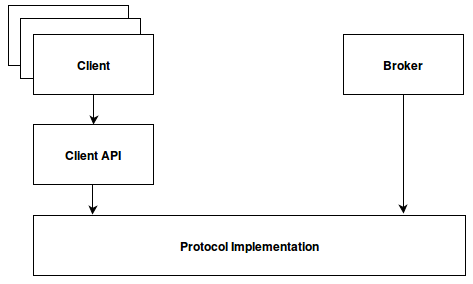
\includegraphics[width=0.6\textwidth]{images/architecture-components.png}
    \caption{Components of the architecture}
    \label{fig:architecture-components.png}
\end{figure}

\section{Protocol}
\label{sec-protocol}

\section{Prototype}
For demonstrating the architecture of this project we implement an architecture
prototype which shows basic functionality of producing a message from a client A
to persisting the message in a  topic specific log at the broker and in turn consuming it from another
client B. It fully implements the produce and fetch request with their
appropriate responses of the Kafka protocol for communication over network.
Therefore the producer and consumer clients are compatible with original Apache
Kafka broker.

The functionality of the architecture prototype can be split in two cases.
Case one covers producing a message and persisting in the brokers log:
\begin{figure}[H]
    \centering
    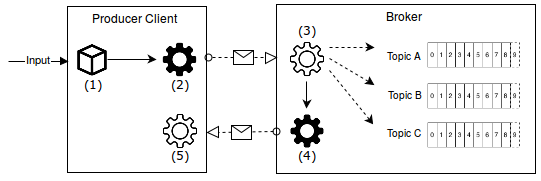
\includegraphics[width=0.9\textwidth]{images/concept_producer.png}
    \caption{Concept of Architecture Prototype Part I}
    \label{fig:conept-producer}
\end{figure}

\begin{table}[h]
\begin{tabular}{ll}
I   & Packing input message in data structure                                                          \\
II  & Serializing of data structure to byte string. The algorithm implements the Kafka protocol.       \\
III & Transmitting byte string via TCP socket over network                                             \\
IV  & Receiving and parsing byte string back to data structure                                         \\
V   & Write Message into topic specific log. The resulting file has same structure than the Kafka Log has.
\end{tabular}
\end{table}

Case two covers the part of consuming from a specific topic. Because Kafka works with 
pull-based consumption, the consumer fetch its messages with a constantly requesting it. 

\begin{figure}[H]
    \centering
   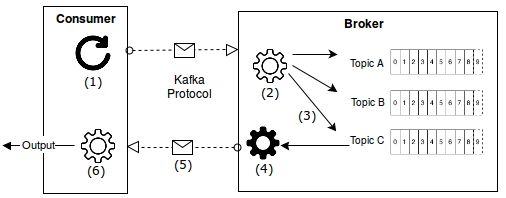
\includegraphics[width=0.6\textwidth]{images/concept_consumer.png}
    \caption{Concept of Architecture Prototype Part II}
    \label{fig:concept-consumer}
\end{figure}

\begin{table}[h]
\begin{tabular}{ll}
I   & Continuously send fetch request to broker implementing Kafka protocol \\
II  & Parse fetch request to data structure                                 \\
III & Read messages from log of specified topic                             \\
IV  & Serialize messages as response into byte string.                      \\
V   & Transmitting byte string back to consumer                             \\
VI  & Parse response from broker to get messages                           
\end{tabular}
\end{table}

\section{Modules}
The application has three main parts namely the broker, protocol implementation
and the client api. 
%Each part is built in its own self-contained cabal package.

\begin{figure}[H]
    \centering
   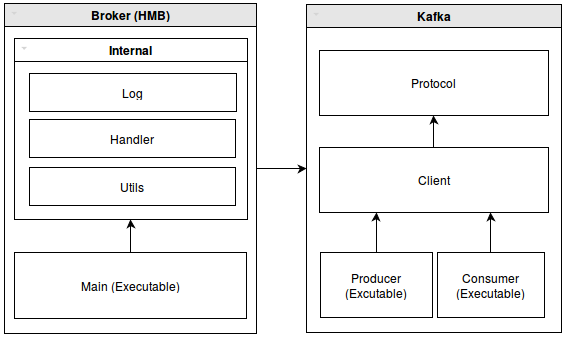
\includegraphics[width=0.85\textwidth]{images/logical-architecture.png}
    \caption{Package structure and dependencies}
    \label{fig:logical-architecture}
\end{figure}



\subsection{Kafka.Protocol}

\subsection{Kafka.Client}

\subsection{Broker.Internal}




